\documentclass[12pt,
border=1pt]{standalone}
\usepackage{pgfplots}
\usepackage{amsmath}
\usepackage{amssymb}

\pgfplotsset{compat=newest,
	width=6cm, height=5cm,
	xtick pos=left, ytick pos=left,
	%            scaled x ticks=real:1e-6,
}
% Kernel 2 FP64
\begin{document}
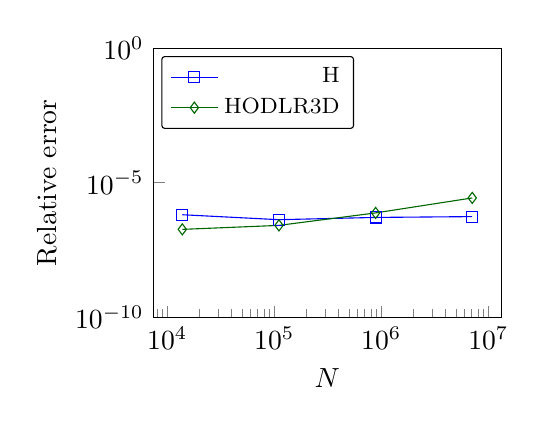
\begin{tikzpicture}
	\begin{axis}[xlabel={$N$},
	ylabel={Relative error},
%		legend pos=south east,
		legend style={
                at={(0.3,0.7)},
               anchor=south,
               legend columns=1,
               cells={anchor=east},
              font=\footnotesize,
               rounded corners=1pt,
               },
		xmode = log,
	    ymode = log,
	   % xmin = 1e3,
	   % xmax = 1e6,
	    ymin = 1e-10,
	    ymax = 1e-0,
	   % xtick={1e-10, 1e-8, 1e-6,  1e-4,  1e-2},
	   % ytick={1e-8, 1e-6,  1e-4,  1e-2, 1e-0}
		]
% 		\addplot[
% 		color=red,
% 		mark=o,
% 		] coordinates {

% (13824,2.031870e-07)
% (110592,1.264230e-07)
% (884736,1.085520e-07)
% (7077888,1.004550e-07)
% 		};
		\addplot[
		color=blue,
		mark=square,
		] coordinates {
(13824,6.480440e-07)
% (64000,4.777380e-07)
(110592,4.242220e-07)
% (512000,6.002560e-07)
(884736,5.146270e-07)
% (4096000,5.592470e-07)
(7077888,5.521490e-07)
		};
		\addplot[
		color=black!60!green,
		mark=diamond,
		] coordinates {
(13824,1.852990e-07)
% (64000,1.977550e-07)
(110592,2.606140e-07)
% (512000,3.842280e-07)
(884736,7.576800e-07)
% (4096000,9.132570e-07)
(7077888,2.725030e-06)
		};
		\legend{H, HODLR3D}
	\end{axis}
\end{tikzpicture}
\end{document}